
\documentclass[a4paper,alpha-refs]{RBCA_v1.0}

\usepackage[portuguese=nohyphenation,english=nohyphenation]{hyphsubst}
% below is defined the main language of the paper - for paper in portuguese you must change "english" by "portuguese".
\usepackage[english]{babel} 
\usepackage{graphicx}
%%% Place your packages here
%%% \usepackage[options]{package}

%%%


%%% title of the paper
\title{A aplicação da derivada na visão computacional: Um estudo sobre a medição de objetos utilizando imagens}

%%% Use the \authfn to add symbols for additional footnotes, if any. 1 is reserved for correspondence emails; then continuing with 2 etc for contributions.
\author[1]{First Author}
\author[2]{Second Author}
\author[2]{Third Author}
\author[2]{Fourth Author}

\affil[1]{First Institution}
\affil[2]{Second Institution}

%%% Author e-mails
\authnote{\authfn{1}first@uni.edu; second@lab.edu; $\cdots$}

%%% "Short" author for running page header
\runningauthor{First et al.}

%%% Paper category:
%%% if in English  : Original paper,  Experience Report     or Tutorial
%%% if in Português: Artigo original, Relato de experiência ou Tutorial
\papercat{Original Paper}

%%% Information about the journal edition and the paper
%%% should only be set by editor
\jvolume{10}           % volume number
\jissue{1}             % issue number
\jyear{2018}           % edition year
\jmonth{April}         % edition month

\setcounter{page}{1}   % number of the first page of the paper
\jpages{1--4}          % paper page numbers
\jid{9999}             % paper ID 

\jrec{yyyy-mm-dd}      % date of article submission
\jrev{yyyy-mm-dd}      % date of final paper revision
\jacc{yyyy-mm-dd}      % date of paper accepted


\begin{document}

\begin{frontmatter}
	
\maketitle

\begin{Abstract} % abstract in english
The Abstract (250 words maximum) should be structured to include the following details: \textbf{Background}, the context and purpose of the study; \textbf{Results}, the main findings; \textbf{Conclusions}, brief summary and potential implications. Please minimize the use of abbreviations and do not cite references in the abstract.
\end{Abstract}

\begin{keywords}
Keyword1; keyword 2; keyword 3 (Three to five keywords representing the main content of the article, in alphabetic order)
\end{keywords}

\begin{resumo} % resumo em português
	O Resumo (com até 250 palavras) deverá ser estruturado para abordar os seguintes detalhes: \textbf{Background}, o contexto e propósito do estudo; \textbf{Resultados}, os principais encontrados; \textbf{Conclusões}, um breve resumo do trabaho e as implicações em potencial. Por favor, evite, na medida do possível, o uso de abreviaturas e não cite referências no resumo.
\end{resumo}

\begin{palavras_chave} % palavras-chave em português 
	Palavra-chave 1; palavra-chave 2; palavra-chave 3 (De três a cinco palavras-chave que representem os principais tópicos do artigo, em ordem alfabética)
\end{palavras_chave}

\end{frontmatter}


\section{Introduction to this Template}

The Revista Brasileira de Computação Aplicada (RBCA) is a \textbf{open access journal} linked to the \href{http://ppgca.upf.br}{Graduate Program in Applied Computing (PPGCA)} of the \href{http://www.upf.br}{University of Passo Fundo}, Brazil. RBCA aims to provide to the scientific community article that present an interdisciplinary perspective of the application of Computing in different areas of knowledge.

This is the \LaTeX{} template for RBCA journal manuscript submissions. \textcolor{red}{Submissions that do not use the format available in this template will be automatically rejected.} 

\textbf{Articles submitted to RBCA should be between 8 and 15 pages and will be published electronically.} The languages accepted by RBCA are Portuguese and English. We alert the authors that the preparation of the manuscript should be made carefully, both in its scientific content and in its grammatical correctness.

There are important commands in the preamble that you will need to modify for your own manuscript. Specify your manuscript's category with the \verb|\papercat{...}| command in the preamble. See the sample code in the preamble for a sample of how author, affiliation and e-mail information can be specified. Information about this edition of RBCA and publication details of the manuscript will be filled out by the journal's editor.

This template has been edited and validated in the \href{http://www.texstudio.org/}{TexStudio\copyright} program and the \href{https://www.overleaf.com/}{Overleaf\copyright} Collaborative Writing and Publishing System. Any questions or problems regarding this template should be reported to the e-mail of the journal (\textcolor{blue}{rbca@upf.br}).

The remainder of this current section will provide some sample \LaTeX{} code for various elements you may want to include in your manuscript.

\section{Processamento de imagem}

O processamento de imagem é um conjunto de operações que separam pontos de interesse e resultam em uma imagem de saída. Utilizando imagens é possível extrair informações sobre as características físicas e geométricas básicas dos objetos, tais como dimensão, área, perímetro e a forma.

Para que um sistema computacional reconheça os elementos de um ambiente ou objeto fotografado é necessário a digitalização de cada ponto. Ou seja, transforma-se o contexto contínuo de "infinitos" átomos em um sistema discreto, isso é, em finitos pontos, denominados como \textit{Picture element} (\textit{pixel}), formando uma imagem. Para isso são necessários dois procedimentos, primeiramente a amostragem e em seguida a quantização. A amostragem consiste na captura de pontos igualmente espaçados no ambiente fotografado, de forma que esses pontos sejam coletados gerando um conjunto de localizações discreta, ou seja, pares ordenados. Já a quantização transforma os valores contínuos da intensidade de cores em valores inteiros contidos em um intervalo. 

A par desse conceito, pode-se representar a imagem como uma função bidimensional denotada por $f$(x,y), tal que x e y são coordenadas de um plano como pode ser visto, obtidas pelo processo de amostragem, e $f$ expressa a intensidade de cinza, provenientes da quantização \citep{ProcDigital}, como pode ser visto na figura \ref{img:lena3d}. Com isso é possível a alocação das intensidades de cada ponto em uma matriz, permitindo aplicação de operações matriciais sobre a fotografia. 

\begin{figure}[h!]
	\centering
	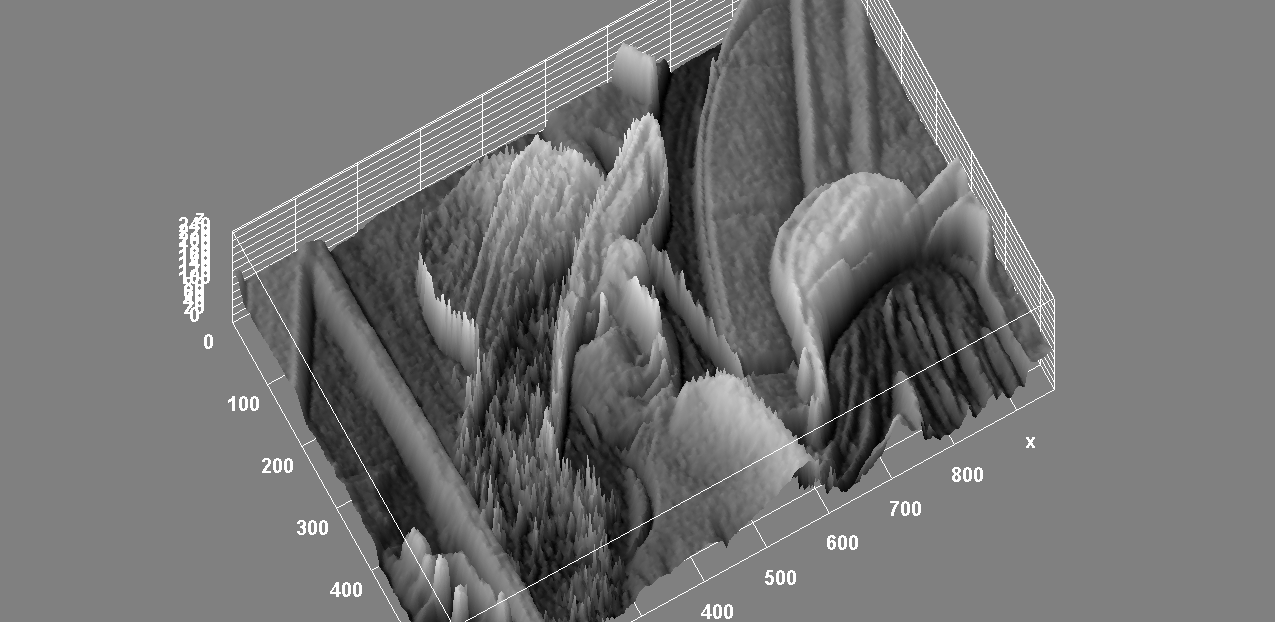
\includegraphics[width=.45\textwidth]{img/img1.png}
	\caption{Representação das dimensões da imagem e a intensidade de cada pixel}
	\label{img:lena3d}
\end{figure}

As imagens são, normalmente, representadas no sistema RGB (do inglês Red, Green and Blue). Isso significa que cada pixel é uma aproximação resultante das intensidades de vermelho, azul e verde. A união das três cores em cada pixel forma uma imagem de 3 bandas \citep{biasi2002desenvolvimento}. Segundo \cite{de2006introduccao} a demonstração da imagem de três bandas pode ser representada pela equação:
\begin{equation}
F(x,y)=F_r(x,y)+F_g(x,y)+F_b(x,y),
\end{equation}
onde $F_r$, $F_g$ e $F_b$ representam respectivamente a intensidade das bandas vermelha, verde e azul. Na área de computação visual adotou-se que a intensidade do pixel igual a 0, em todas as bandas, representa o preto, enquanto 255 representa o branco. Todas as outras cores são variações nesse intervalo. 

Assim, o processamento se inicia transformando a imagem formada pelas bandas RGB em tons de cinza, como visto na Figura \ref{img:lenargb}. 
\begin{figure}[h!]
	\centering
	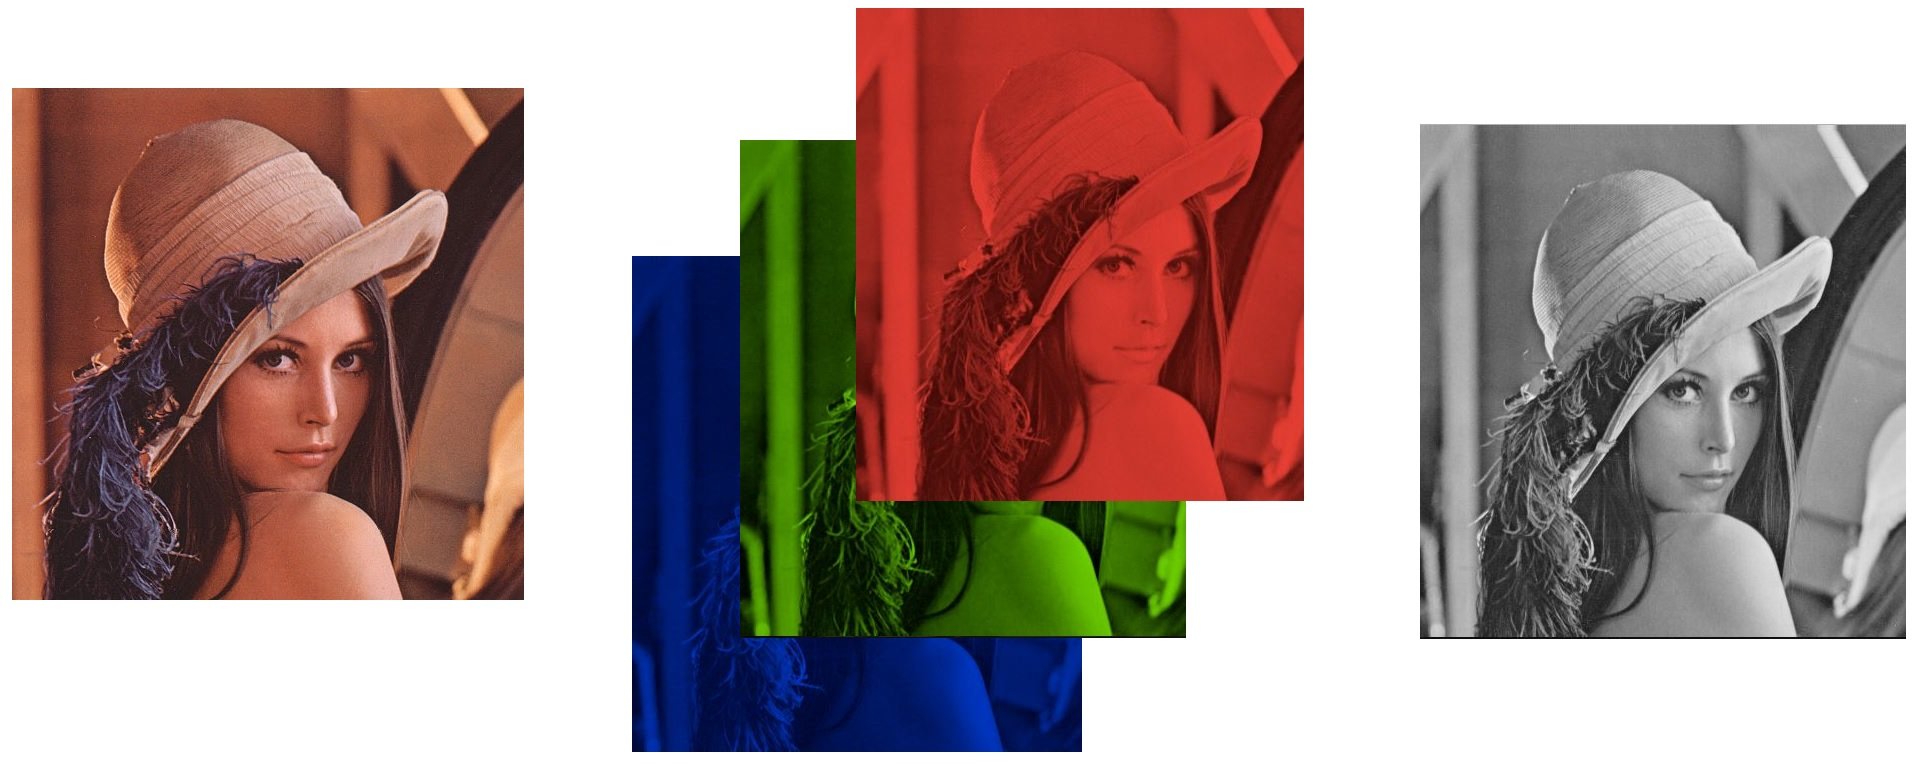
\includegraphics[width=.5\textwidth]{img/lenna_rgb_gray.jpg}
	\caption{Representação de uma imagem nas bandas RGB e em escala de cinza}
	\label{img:lenargb}
\end{figure}

Essa transformação será necessário para analisar apenas como uma variação de cinza. Segundo a documentação oficial dos desenvolvedores da biblioteca Opencv a transformação aplicada é baseada em uma média ponderada das componentes RGB de cada pixel, dada pela fórmula:
\begin{eqnarray*}
F(x,y)=(0,299*F_r(x,y))+(0,587*F_g(x,y)) \\ +(0,114*F_b(x,y))
\end{eqnarray*} 

***Segundo \cite{de2006introduccao} existem duas classificações importantes quando se trata de operações que manipulam de forma direta o pixel: as operações pontuais e as operações locais ou por máscaras. Nas operações pontuais cada pixel é tratado de forma independente. Já nas operações locais ou por máscara, o valor de saída depende de um conjunto de pixels vizinhos. É importante salientar, que as máscaras são matrizes com dimensões pequenas em que o pixel a ser tratado é posicionado no centro da matriz de operação e o resultado é um novo valor na mesma posição.

Com essas definições torna-se possível aplicar o método para a detecção de borda desenvolvido por John Canny. A imagem de saída resultante da aplicação desse método é do tipo imagem binária, pois os elementos variam entre 0 ou 1, de forma que 1 representa a presença de borda em um determinado pixel, na Figura \ref{img:lenaborda} a presença de borda é representada pela cor branca. 

\begin{figure}[h!]
	\centering
	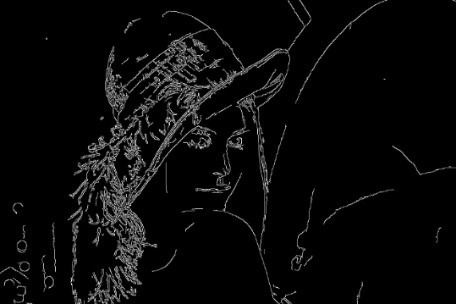
\includegraphics[width=.3\textwidth]{img/img9.jpg}
	\caption{Representação da borda de uma imagem}
	\label{img:lenaborda}
\end{figure}

\section{Métodos Canny para detecção de bordas}
\subsection{Suavização Gaussiana}

\subsection{Detecção do gradiente}

Após a suavização de ruídos na imagem, os métodos de detecção das bordas precisam de ferramentas que permitam localizar variações bruscas de cores. É nesse momento que o conceito de derivada é utilizado por meio do gradiente.

O gradiente é um vetor bidimensional que ele representa a taxa de variação da função $f$ na posição (x,y). Ele é dado por $\nabla f$ :
\begin{equation}
\nabla f = (Gx,Gy) = \left(\frac{\partial f}{\partial x},\frac{\partial f}{\partial y}\right).
\label{eq:gradiente}
\end{equation}
É necessário utilizar esse tipo de ferramenta uma vez que a imagem é representada por uma função de duas dimensões, podendo ocorrer variações de intensidade de cores tanto em relação ao eixo x quanto ao eixo y. 

No contexto do processamento de imagem, o gradiente fornecerá a direção e o sentido da variação de intensidades de cores entre um pixel e seus vizinhos por meio do ângulo $\alpha$ obtido pela equação: 
\begin{equation}
\alpha (x,y) = \arctan \left(\frac{Gx}{Gy}\right).
\label{eq:angulo}
\end{equation}
A direção do gradiente é importante uma vez que ele é ortogonal à borda, como é possível visualizar na Figura \ref{img:exemplo1}.
\begin{figure}[h!]
	\centering
	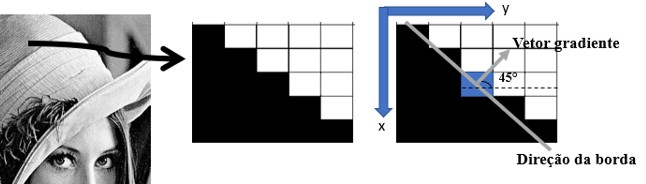
\includegraphics[width=.5\textwidth]{img/1-gradiente.jpg}
	\caption{Vetor gradiente representado sobre a imagem}
	\label{img:exemplo1}
\end{figure}

Além disso, a magnitude, que indica intensidade da variação, é dada por:

\begin{equation}
M = M(x,y) = \sqrt{(Gx)^2 + (Gy)^2} 
\label{eq:modulo}
\end{equation}

***O gradiente é uma importante ferramenta para encontrar as bordas, entretanto, como aplicar a derivada em um sistema com valores digitais? Para isso se utiliza uma aproximação da derivada parcial, que é aplicada pixel-a-pixel. Como já visto, a derivada é conceituada como a variação instantânea de uma dada função, generalizando esse conceito pode-se chegar às seguintes equações:
\begin{equation}
G_x = \frac{\partial f(x,y)}{\partial x} = f(x + 1,y) - f(x,y)
\label{eq:gradientex}	
\end{equation}
\begin{equation}
G_y = \frac{\partial f(x,y)}{\partial y} = f(x ,y+ 1) - f(x,y)
\label{eq:gradientey}
\end{equation}

Isso significa que a diferenciação em um elemento da imagem pode ser vista como a diferença das intensidades dos elementos vizinhos. Dessa forma, o resultado da aproximação deve ser zero em locais onde a intensidade é constante,  e diferente de zero nos pontos onde ocorrem variações de cores, satisfazendo os conceitos de derivada.

É importante ressaltar que as formas apresentadas nas equações \ref{eq:gradientex} e \ref{eq:gradientey} para a obtenção do gradiente não são suficientes quando se trata de bordas diagonais, uma vez que a intensidade de cor dos pixeis vizinhos na diagonal não são considerados. Uma forma de solucionar esse problema é construir uma máscara de $2$ dimensões que detecte variações de todos os 8 vizinhos. Segundo \cite{ProcDigital} essas máscaras recebem o nome de \textit{Operadores de Prewitt} e podem ser vistas na Figura \ref{img:mascara} (b). O método de Canny utiliza o \textit{Operador de Sobel}, o qual valoriza os pixeis mais próximos por meio de um peso, representado na Figura \ref{img:mascara} (c).

\begin{figure}[h!]
	\centering
	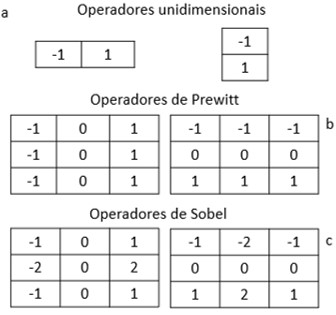
\includegraphics[width=.3\textwidth]{img/mascara.jpg}
	\caption{Matrizes representantes dos operadores diferenciais}
	\label{img:mascara}
\end{figure}

Um exemplo da aplicação do \textit{Operador de Sobel} pode ser visualizado na figura \ref{img:gradiente}. A Figura \ref{img:gradiente}(a) é constituída apenas por duas tonalidades de cinza, 0 (preto) e 255 (branco). Dessa forma, a variação é detectada exatamente quando há a troca de cores, (figuras \ref{img:gradiente} (b) e (c)), que representam os gradientes na direção x e y respectivamente. Essa detecção é vista como uma linha branca traçada na diagonal, ou seja, quando a derivada é máxima.

\begin{figure}[h!]
	\centering
	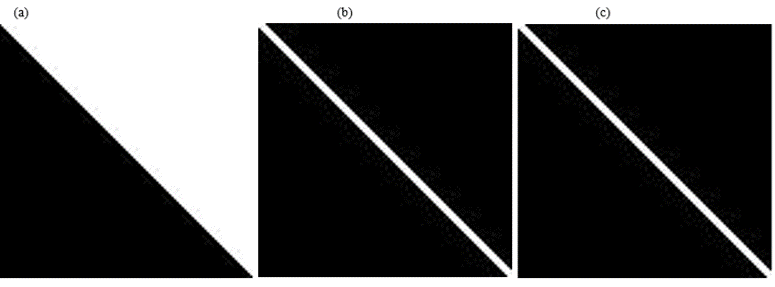
\includegraphics[width=.35\textwidth]{img/gradiente.png}
	\caption{Representação da aplicação do gradiente na direção de x (b) e y (c)}
	\label{img:gradiente}
\end{figure}

Como forma de demonstrar o método de detecção da variação de cores, suponha que se deseja detectar a existência de uma borda no pixel destacado (na cor azul) - Figura \ref{img:Primeira}. Suponha também que a cor escura seja igual a 0 e a cor clara seja 255. O primeiro passo é centralizar o pixel com o centro do \textit{Operador de Sobel}.

\begin{figure}[h!]
	\centering
	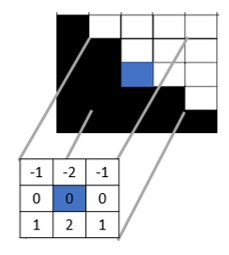
\includegraphics[width=.3\textwidth]{img/1im.jpg}
	\caption{Centralizando pixel com o Operador de Sobel}
	\label{img:Primeira}
\end{figure}

***Multiplica-se assim o pixel analisado e seus 8 vizinhos pelo valor correspondente à sua posição no operador. Esse processo resultará em uma matriz com as mesmas dimensões do operador. O próximo passo é fazer a somatória dos elementos desse \textit{array} resultante, detectando dessa forma a intensidade do gradiente em uma das direções. Por fim, o valor obtido é colocado, na mesma posição do pixel que foi estudado, em uma nova matriz, denominada como matriz de gradientes, o que pode ser observado na figura \ref{img:grady}. 

\begin{figure}[h!]
	\centering
	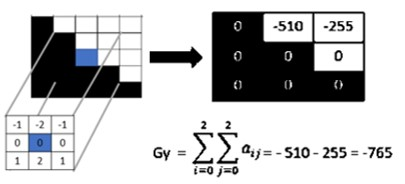
\includegraphics[width=.3\textwidth]{img/grady.jpg}
	\caption{Encontrando a intensidade do gradiente}
	\label{img:grady}
\end{figure}

Realizando os mesmos procedimentos com o operador em x, obtém-se $Gx = 765$. Utilizando as operações por meio da equação \ref{eq:angulo}, constata-se que $\alpha = -45$° o que equivale a 135° considerando o sentido anti-horário. Por fim, pela equação \ref{eq:modulo} é possível deduzir um valor representante da variação nas duas dimensões. Realizando as contas obtemos que $M = 765\sqrt{2}$. Esse valor é alocado em uma nova matriz, na posição correspondente ao pixel estudado.

Após obter o gradiente em todos os pixeis em relação aos seus vizinhos, se inicia o processo de filtragem dos pontos que serão considerados como bordas. Isso significa que os próximos passos do método de Canny serão responsáveis por encontrar os valores máximos da função gradiente, uma vez que esses serão as bordas.

\subsection{Supressão do não máximo}

O primeiro passo para a filtragem dos valores obtidos por meio do gradiente é a supressão do não máximo. É nesse momento que se utiliza a orientação, ou seja, o ângulo do gradiente, de forma que será anulado todos os valores não máximos nessa direção.

Inicialmente, é necessário fazer um arredondamento do ângulo obtido por meio do gradiente. Isso se justifica pois, como as imagens são armazenadas como matrizes não é possível obter um ângulo de 43°, por exemplo, entre dois pixeis. Os possíveis valores de vizinhança para um ponto, sempre serão múltiplos de 45°, ou seja, 0° e 180° para os vizinhos a direita e esquerda respectivamente; 90° e 270° para os pixeis superior e inferior ao ponto; 45° e 225° para os vizinhos na diagonal à direita; e 135° e 315° para os vizinhos à diagonal a esquerda. Todos os valores diferentes desses são arredondados para o mais próximo. Esse arredondamento é tratado automaticamente pela função utilizada no algoritmo desenvolvido nesse artigo.

Após isso, o método de Canny segue todas as direções dos gradiente e vai anulando os valores não máximos nessas orientações. Como visto, a direção do gradiente é ortogonal à borda. Assim, a supressão do não máximo não afetará a borda, mas os valores ao redor dela, uma vez que é na borda que há a maior intensidade do gradiente. Dessa forma, a supressão do não máximo possibilitará a detecção de possíveis pixeis representantes de bordas. 

Aplicando a derivada em todos os pixeis da Figura \ref{img:Primeira} obtemos os valores da magnitude do gradiente, como pode ser visto na Figura \ref{img:imgSu} (a). Aplicando a supressão do não máximo na direção do gradiente obtemos uma redução dos valores possíveis para a borda- Figura \ref{img:imgSu} (b).   

\begin{figure}[h!]
	\centering
	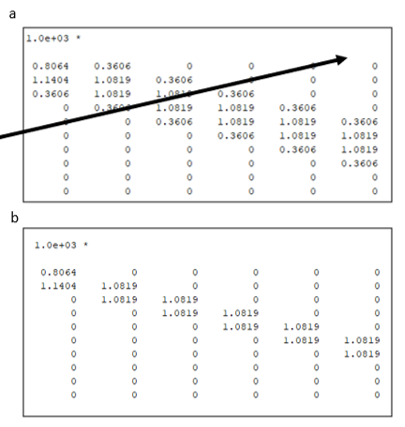
\includegraphics[width=.5\textwidth]{img/imgSu.png}
	\caption{Aplicando supressão do não máximo na matriz resultante do gradiente}
	\label{img:imgSu}
\end{figure}

\subsection{Limiarização}

O processo final da detecção de bordas elaborado por Canny é a limiarização. Essa etapa consiste em separar a imagem em duas partes: a primeira representa a região de interesse (borda), e a segunda representa áreas não desejadas como ruídos, bordas falsas, fundos ou preenchimentos dos objetos.  Isso significa que esse processo se resume em categorizar a intensidade cinza por meio de um valor limiar, de forma que os valores abaixo e acima desse limite são tratados de maneira diferente.
 
Desse modo o processo de limiarização produz uma imagem binária bem definida, ou seja, os valores maiores que o limiar recebem a intensidade 1, valor máximo. Por outro lado, todas as outras intensidades são trocadas por zero. Segundo \cite{ProcDigital} esse processo é denominado binarização da imagem que pode ser definida matematicamente como a equação:
\begin{equation}
G(x,y) = \\ 
\left\{
\begin{array}{cc}
 1 , \ \mbox{se} \;\;\; f(x,y)>T \\
 0 , \ \mbox{se} \;\;\; f(x,y) \leq T \\
\end{array}
\right.,
\label{eq:limi}	
\end{equation}     
onde f(x,y) é a imagem de entrada, T é o valor de limiar e G(x, y) é a imagem de saída ou limiarizada. Podemos observar que na equação \ref{eq:limi} os valores maiores que o limiar são considerados como borda, e os valores abaixo desse limiar são considerados como áreas não desejadas.

Aplicando a limiarização com $T =  1.0819 * 10^3$ e com $T =  1.1404 * 10^3$  na Figura \ref{img:imgSu} (b), obtemos os resultados da Figura \ref{img:imgLi}(a) e (b) , respectivamente. Esse valor de limiar é a segunda aproximação que o sistema de Canny utiliza, ou seja, não há um resultado concreto e único. Cada ambiente possui variáveis que influencia nesse limiar como iluminação, quantidade de ruídos e etc. No contexto do algoritmo desenvolvido, é função do usuário fazer uma aproximação de limiar com base nas suas necessidades.

\begin{figure}[h!]
	\centering
	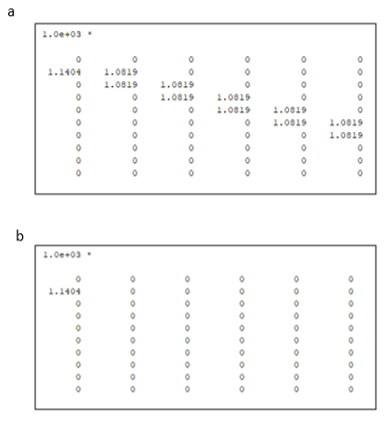
\includegraphics[width=.5\textwidth]{img/imgLi.png}
	\caption{Aplicando a limiarização na matriz resultante da supressão do não máximo}
	\label{img:imgLi}
\end{figure}

A figura \ref{img:imgLi2} mostra como o limiar pode afetar na borda. Em (a) está representado a imagem resultante do limiar mais baixo e em (b) a imagem resultante do limiar mais alto.  

\begin{figure}[h!]
	\centering
	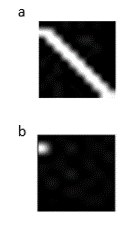
\includegraphics[width=.2\textwidth]{img/imgLi2.png}
	\caption{Imagem resultante das limiarizações}
	\label{img:imgLi2}
\end{figure}
 
\section{Desenvolvimento do algoritmo}

Como apresentado, o objetivo geral deste artigo é demonstrar de forma prática a aplicação do cálculo de derivadas na área da Engenharia de Computação. Com esse intuito, foram realizadas pesquisas e experimentações para aprofundar o conhecimento em processamento de imagens. Além disso, um dos objetivos específicos foi desenvolver um algoritmo capaz de encontrar as bordas de um objeto em uma imagem e com isso retornar dados da sua medição, demonstrando uma aplicação dos dados extraídos de uma imagem processada.

A detecção da variação de intensidade em imagens é algo canônico na visão computacional
\citep{canny1983variational}, e é baseado nos estudos do método aplicado por John Canny para detecção de bordas que foram realizadas as experimentações. Retomando o objetivo geral do trabalho, o entendimento do método Canny foi necessário, dado que este se baseia na aplicação da primeira derivada da função Gaussiana.

A primeira etapa foi dedicada a desenvolver um algoritmo que através da manipulação da matriz de uma imagem, retornasse uma matriz resultante apenas com elementos binários. Utilizando a biblioteca OpenCV, foi desenvolvido um algoritmo que recebe uma imagem e a salva na forma matricial, onde cada pixel representa um elemento da matriz. O número atribuído a esse pixel, ou seja, ao elemento dessa matriz, é um valor do sistema RGB. Na sequência, transformam-se os valores dos canais RGB em um único representante na escala de cinza. Essa modificação é necessária para diminuir as variações entre as cores dos pixeis. Por fim, é aplicado o método Canny, que é capaz de identificar mudanças na intensidade dos pixeis da imagem para detectar a presença de bordas.

\section{Resultados}

Retomando um dos objetivos específicos deste trabalho, utilizamos a matriz binária gerada após aplicação do método Canny para realizar a medição de um objeto contido na imagem. Interpretando a matriz resultante como um sistema de coordenadas, onde as colunas representam o eixo x e as linhas representam o eixo y, foram criadas duas funções:

- A primeira função, busca pelo primeiro e pelo último elemento (x, y) da matriz cujo valor seja 1, ou seja, presença de borda. Subtraindo o componente y do ultimo elemento, pelo componente y do primeiro elemento, obtêm-se a altura em pixeis do objeto. Essa função limita-se a medir objetos sem que haja aplicação de rotações.

- A segunda função, faz uma varredura na matriz em sentidos opostos, encontrando duas quinas no objeto. Dessa maneira, com a informação da coordenada (x, y) das quinas, utilizou-se o conceito de distância entre dois pontos para encontrar o valor em pixeis de uma quina à outra. Essa função limita-se a medir objetos com quinas bem definidas, quando a medida é o diâmetro, por exemplo, utiliza-se o método citado anteriormente. Rotações que não envolvam o eixo de profundidade são medidas sem que haja danos ao resultado. 

\begin{figure}[h!]
	\centering
	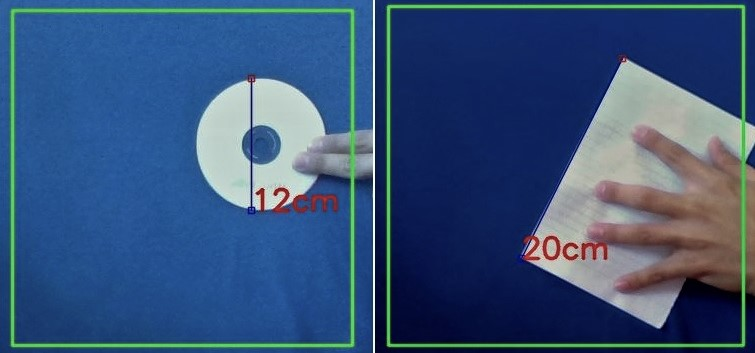
\includegraphics[width=.3\textwidth]{img/01-IMAGEM1.jpg}
	\caption{Demonstração dos métodos de medição}
	\label{img:img1}
\end{figure}

Foram realizadas diversas experimentações para constatar a correlação entre a medida em pixeis, e a medida real do objeto em milímetros. Neste processo controlaram-se algumas variáveis, como: a distância do objeto à câmera; a rotação do objeto; e o processo de limiarização do método Canny.

\begin{figure}[h!]
	\centering
	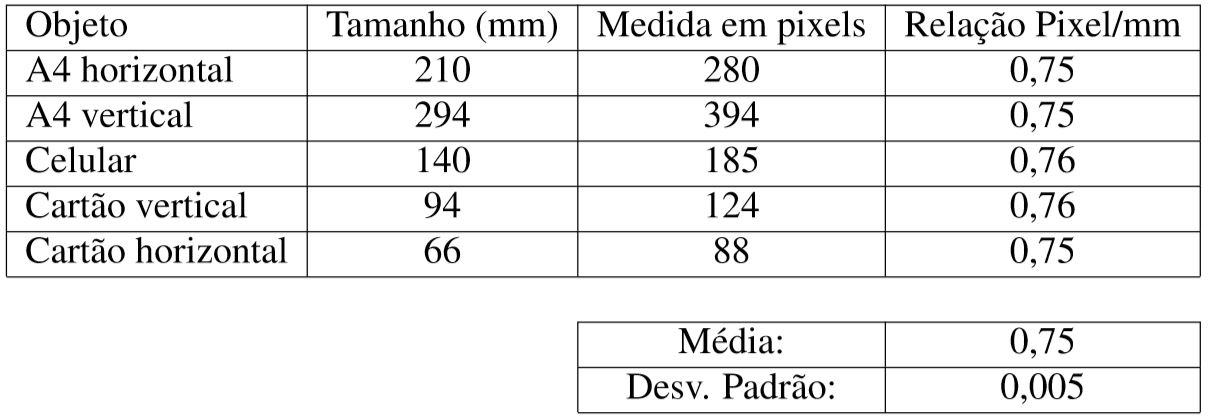
\includegraphics[width=.3\textwidth]{img/02-TABELA1.JPG}
	\caption{Resultados das medições realizadas a 500mm de distância}
	\label{img:tabela1}
\end{figure}

\begin{figure}[h!]
	\centering
	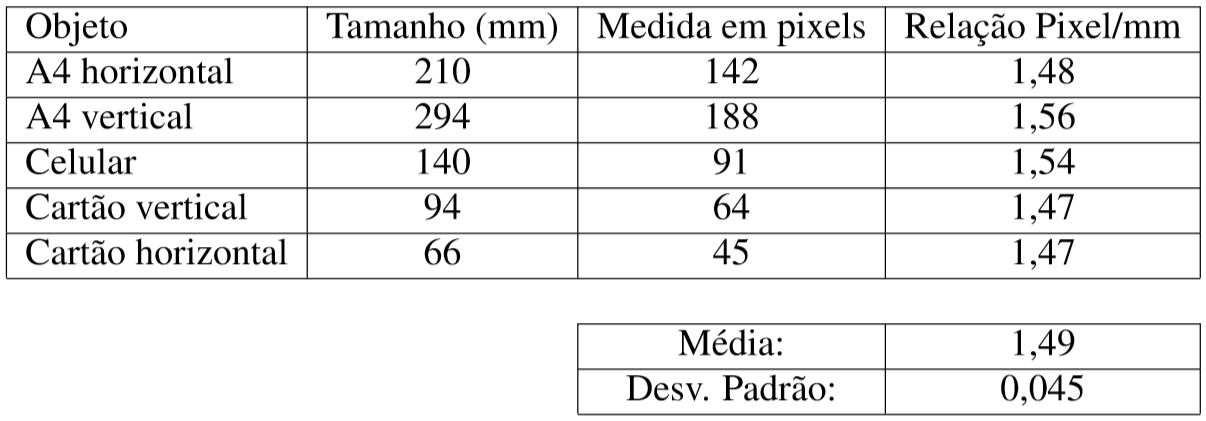
\includegraphics[width=.3\textwidth]{img/03-TABELA2.JPG}
	\caption{Resultados das medições realizadas a 1000mm de distância}
	\label{img:tabela2}
\end{figure}

Como pode ser observado na figura \ref{img:tabela1}, o desvio padrão da relação pixel/milímetros é bem inferior àquela constatada na figura \ref{img:tabela2}. Isso indica que quanto menor a distância entre a câmera e o objeto medido, maior será a repetitividade do processo, assim como melhor será a precisão. Isso está relacionado com a perda de detalhes do objeto ao afastá-lo da câmera. 

Buscando realizar medições em tempo real, foi necessário criar uma etapa para estabelecer uma relação inicial entre pixeis e centímetros a ser mantida durante a medição de novos objetos. Este processo consiste na utilização de um objeto com dimensões conhecidas, e a partir da medição deste objeto, dada em pixeis, computar a relação entre pixel e centímetro a ser mantida.

\begin{figure}[h!]
	\centering
	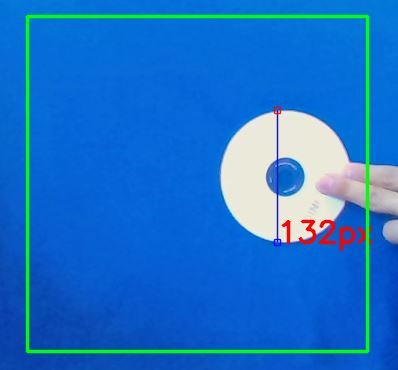
\includegraphics[width=.3\textwidth]{img/04-IMAGEM2.JPG}
	\caption{Computando a altura em pixeis para ser utilizado como referência}
	\label{img:img2}
\end{figure}

A imagem \ref{img:img2}, o diâmetro do CD foi equivalente à 132 pixeis. Como um CD padrão tem diâmetro de 12,0 centímetros, o software computou a relação pixel/centímetro equivalente à aproximadamente 0,091 centímetros por pixel. Esta relação foi estabelecida com a câmera a uma distância de 750 milímetros do objeto, e, portanto, mantida para as demais medições.

Como as bordas que não representam o objeto, e as bordas do objeto são armazenadas da mesma maneira, ao analisar a imagem completa, a presença de detalhes indesejados impedia o processo de medição. Essa situação era devido ao fato de o algoritmo procurar o primeiro e o último elemento da matriz que representasse borda, e ao encontrar falsas bordas, ou bordas que não representam o objeto, falhas eram geradas. Percebido isso, foi desenvolvida uma nova função no programa com a função de delimitar a região de interesse. Esta função tem como objetivo reduzir a área de busca por bordas, transformando a matriz da imagem em uma matriz menor.

\begin{figure}[h!]
	\centering
	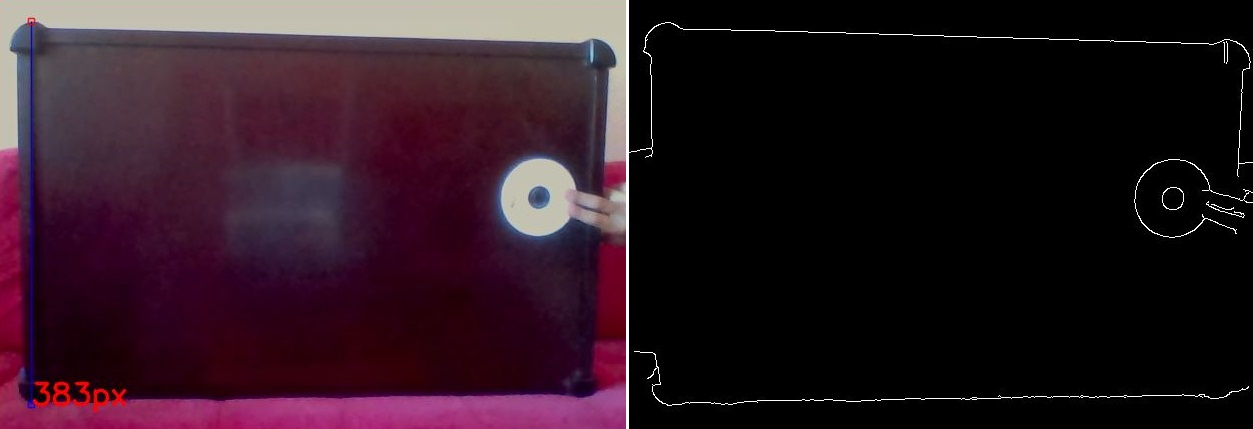
\includegraphics[width=.5\textwidth]{img/05-IMAGEM3.jpg}
	\caption{Detecção de borda sem a região de interesse}
	\label{img:img3}
\end{figure}

\begin{figure}[h!]
	\centering
	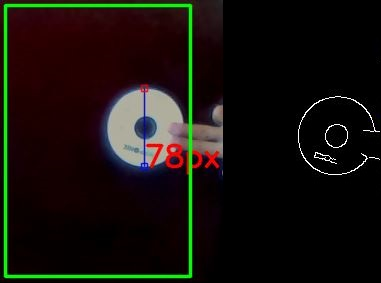
\includegraphics[width=.3\textwidth]{img/06-IMAGEM4.jpg}
	\caption{Detecção de borda dentro da região de interesse}
	\label{img:img4}
\end{figure}

Como pode ser observado na figura \ref{img:img3}, em que não há delimitação da área de busca, o algoritmo retornou uma altura em pixeis equivalente à 383px. Já na imagem \ref{img:img4}, a região de busca por bordas corresponde à área interna do retângulo de contorno verde, isso significa que somente o que estiver compreendido na região de interesse será analisado.

Além do problema com a região de interesse, houve também a necessidade de permitir que o usuário pudesse modificar, quando necessário, a limiarização desejada para o processo. Pois, a aplicação da limiarização é difícil e envolve experimentação. “A permanência de falsas bordas, após a limiarização, pode ter como motivo a escolha de um limiar baixo, ou alto demais” (Do Vale and DAL POZ 2002,p. 9). Na imagem \ref{img:img4} as bordas ficam restritas ao objeto, já na figura \ref{img:img5}, ocorre a presença de falsas bordas, sendo possível perceber o impacto de uma limiarização mal aplicada, o que interfere na medição.

\begin{figure}[h!]
	\centering
	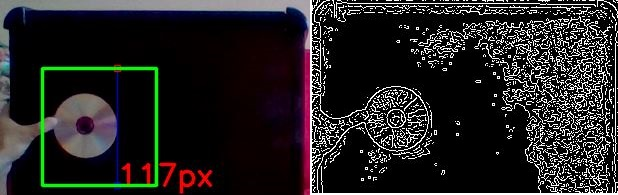
\includegraphics[width=.5\textwidth]{img/07-IMAGEM5.jpg}
	\caption{Detecção de borda com limiarização mal aplicada}
	\label{img:img5}
\end{figure}

Por fim, reduzindo a região de interesse, e permitindo a limiarização durante o processo de medição, o algoritmo foi capaz de retornar medições dos objetos com uma precisão de 0,0962 centímetro, ou seja, inferior à 1 milímetro (vide Figura \ref{img:tabela3}). Esse é um resultado aceitável, visto que se buscava a demonstração de uma utilização dos dados de saída do método de detecção de borda. Porém, o fato de trabalharmos com uma câmera 2D, implicou na perda de percepção de profundidade. Logo, quando há rotação do objeto em profundidade a medição passa a se invalidar. Aprofundar os cálculos para encontrar medições do objeto independente da rotação, é uma das possíveis vertentes que este trabalho poderá seguir, portanto não será abordada essa variável de processo.

\begin{figure}[h!]
	\centering
	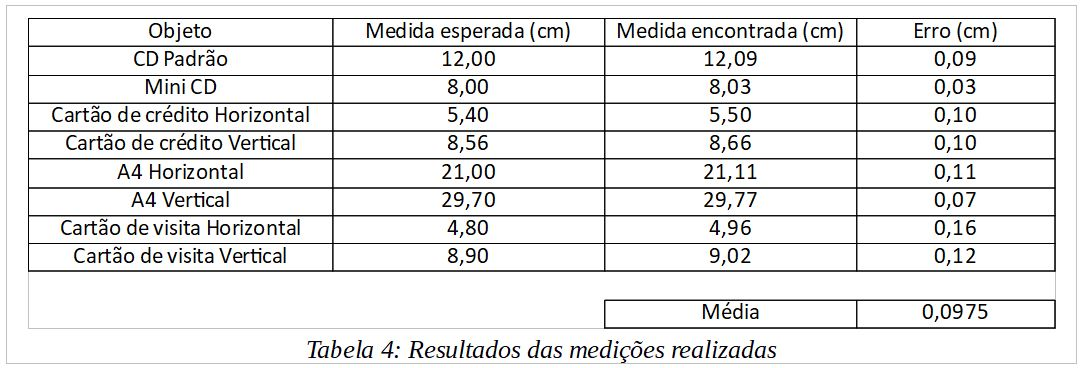
\includegraphics[width=.5\textwidth]{img/T4.JPG}
	\caption{Resultados de medições}
	\label{img:tabela3}
\end{figure}

\bibliography{references} 

\end{document}
